% Canonical paper: Beyond PO and PA (observation-quality levels).
% Dataset-style draft (MallorcaPlant): archived in main.tex — not primary.
\documentclass{article}
\usepackage{graphicx} % Required for inserting images
\usepackage{amsmath}

\title{Beyond presence-only and presence-absence data: observation-quality levels for plant SDMs on Mallorca}
\author{Iv\'an Cort\'es-Fern\'andez \and Pablo Ubilla Pavez \and Diego Marcos}
\date{2026}

\begin{document}

\maketitle

\section{Abstract}

Research questions (Beyond PO vs PA --- observation-quality \emph{levels}):
(1) Which level informs rare vs common species, and does presence-only rarify taxa that are common on complete atlas cells?
(2) How much does incomplete presence--absence (PAU) add beyond validated/unvalidated presence-only?
(3) What mix of PAU/POV/POU is optimal for \emph{finding} species (inventory) versus transferring to PAC (SDM)?

We argue that binary PO vs PA is insufficient. Mallorca supports four levels: complete grid PA (PAC), incomplete grid PA (PAU), validated PO (POV), and unvalidated PO (POU). Records were curated to the Mallorca flora $\cup$ official alien list. Analyses combine descriptive rarity and species-accumulation mixes with multi-species deep SDMs trained on PAU/POV/POU and evaluated on PAC at cell grain (\texttt{grouped}). Locked curated metrics and figures: \texttt{output/curated/} (do not invent numbers in prose until copied from those files).

\section{Keywords}

species distribution model; deep learning; transfer learning; citizen science; atlas data; Mallorca; plant biodiversity


\section{Introduction}

Species Distribution Models (SDMs) have become fundamental tools for understanding macroecological patterns, assessing biogeography, and guiding biodiversity conservation strategies (). However, the predictive performance, accuracy, and transferability of these models are critically based on the volume, quality, and representativeness of the occurrence data used for their calibration (). In recent decades, spatial ecology has greatly benefited from open-access global databases such as the Global Biodiversity Information Facility (GBIF), which aggregates millions of presence-only records derived from museum collections, herbaria, and opportunistic observations. Although these platforms provide unprecedented global coverage, modeling based exclusively on presence-only data faces severe methodological limitations,, including high rates of duplicates \cite{insects16080769}. 

Opportunistic records are intrinsically affected by strong spatial and taxonomic biases; they tend to be heavily concentrated in easily accessible areas—such as near roads or research centers—and often overrepresent conspicuous or perennial plant species while neglecting rare or cryptic taxa \cite{insects16080769}. Crucially, GBIF data lack true absence records, forcing modelers to generate analytical pseudo-absences or background points. If not calibrated carefully, the selection of pseudo-absences can introduce significant uncertainty, inflate false positives, and distort the estimated ecological niche. In contrast, structured biological inventories and exhaustive floras offer highly rigorous, standardized data \cite{barbet2012selecting,chefaoui2008assessing,phillips2009sample,lobo2010uncertain}. These datasets not only provide taxonomically curated presences but, by design, allow for the reliable inference of true absences at local and regional scales. The inclusion of presence-absence data provides a much cleaner ecological signal, allowing models to accurately differentiate whether a species is absent due to abiotic physiological limitations or due to dispersal barriers. However, the primary obstacle with exhaustive floristic inventories is the massive investment of time, expertise, and funding they require, which inevitably results in a geographically fragmented coverage that leaves vast territorial gaps.
To complement these traditional data sources, the exponential growth of citizen science platforms (e.g., iNaturalist) provides a rapidly accumulating stream of biodiversity observations. When rigorously filtered and validated, citizen science data can significantly expand spatial and environmental coverage, capturing records in undersampled regions and providing independent occurrences that academic sampling might miss.
To overcome the dichotomy between massive but biased presence-only data and high-quality but spatially restricted presence-absence data, the current frontier in ecological modeling relies on Integrated Species Distribution Models (IDMs), or data fusion frameworks \cite{isaac2020data,Datafusion2025} , which includes data pooling, independent model combinations, auxiliary data integration, informed priors and model complete integration \cite{fletcher2019practical}. IDMs allow for the statistical hybridization of different data types, seamlessly combining structured presence-absence data from floristic inventories with unstructured, presence-only records from GBIF and validated citizen science. This integration capitalizes on the unique strengths of each source: the exhaustive inventories provide the necessary statistical anchor to accurately delimit habitat suitability and account for detection probability, while the massive opportunistic datasets fill spatial gaps and broaden the sampled environmental gradients \cite{isaac2020data,Grattarola2023}.
In this context, the present article aims to evaluate the predictive performance of plant SDMs by integrating three distinct dimensions of spatial data: (1) historical and opportunistic presences from GBIF, (2) structured floristic inventories (presences and true absences) differentiating between finished and non-finished sampled areas, and (3) validated presences derived from citizen science. We hypothesize that this multi-source data fusion approach will effectively mitigate the individual sampling biases of each dataset, optimize the delineation of the bioclimatic niche, and generate substantially more robust and reliable biogeographical projections for plant species.

\section{Material and methods}

\subsection{Study area}

\subsection{Biodiversity Data gathering}

Data about Plantae was gathered from the study area, differentiating into various subgroups:

\begin{itemize}
    \item Inventories at 500x500m or 1x1km carried out in long sampling periods (>3 years) and in which authors observed saturation indicators of taxa diversity (here after Presence-Absence-Complete data or \textbf{PAC}). This data was present in GBIF, and authors were contacted to dilucidate 
    \item Inventories at 500x500m or 1x1km carried out in short sampling periods (<3 years) and in which authors not observed saturation indicators of taxa diversity (here after Presence-Absence-Uncomplete data or \textbf{PAU})
    \item Presence-Only data coming from Biodibal, a citizen-science platform where ocurrences are validated by experts previously to their inclusion in de database (hereafter Presence-Only Validated data or \textbf{POV})
    \item Presence-Only data coming from GBIF, with indicated coordinate uncertainy that not exceeds 1000m and which have not been reviewd by experts (hereafter Presence-ONly Unvalidated data or \textbf{POU})
\end{itemize}

To differentiate between PA and PO data, coordinates uncertainties of 707m were used as an indicator of the PA nature of data (707 is de radious required to include a square of 1km in a circle that contains all potential locations of the taxa) and confirmed by data authors. 

Table 1. 

\begin{table}[ht]
\centering
\caption{Definición de modelos, verosimilitud y función de intensidad para los distintos tipos de datos}
\begin{tabular}{llll}
\hline
\textbf{Tipo de datos} & \textbf{Modelo} & \textbf{Verosimilitud} & \textbf{Función de intensidad} \\
\hline
PAC & Presencia--ausencia completa &
$Y{\text{PA}} \sim \text{Bernoulli}\big(f(\lambda{\text{PA}})\big)$ &
$\log(\lambda{\text{PA}})=\alpha{\text{PA}}+\beta x + g(s)$ \\

PAU & Presencia--ausencia incompleta &
$Y{\text{PA}} \sim \text{Bernoulli}\big(f(\lambda{\text{PA}})\big)$ &
$\log(\lambda{\text{PA}})=\alpha{\text{PA}}+\beta x + g(s) + h(s)$ \\

POV & Presencia--solo validada &
$Y{\text{PO}} \sim \text{Poisson}(\lambda{\text{PO}})$ &
$\log(\lambda{\text{PO}})=\alpha{\text{PO}}+\beta x + g(s)$ \\

POU & Presencia--solo no validada &
$Y{\text{PO}} \sim \text{Poisson}(\lambda{\text{PO}})$ &
$\log(\lambda{\text{PO}})=\alpha{\text{PO}}+\beta x + g(s) + h(s)$ \\

\hline
\end{tabular}
\end{table}

Taxonomy was unified prior to analysis using GBIF backbone. To do so, taxonid from each taxon name was extracted using pygbif library(). Then, unfound taxa were manually assigned. After that, the dataset was taxonomically filtered to exclude taxa belonging to several orders and families that were outside the scope of the study. Specifically, records assigned to the orders Bryales, Bryopsidales, Ceramiales, Cladophorales, Corallinales, Dasycladales, Dicranales, Fossombroniales, Funariales, Hypnales, Jungermanniales, Marchantiales, Nemaliales, Pelliales, Peyssonneliales, Porellales, Pottiales, Scouleriales and Siphonocladales were removed. In addition, taxa belonging to the families Posidoniaceae, Potamogetonaceae, Ulvaceae, Phyllophoraceae, Ceratophyllaceae, Anadyomenaceae, Zosteraceae, Ruppiaceae, Bonnemaisoniaceae, Cymodoceaceae and Hydrocharitaceae were excluded. These filters were applied to remove non-target groups (e.g., bryophytes, macroalgae and marine angiosperms) and retain only the taxa relevant to the ecological analyses performed. Analyses was performed as species level. Points in the sea were omitted for the analysis, as only terrestrial plants were considered.

\paragraph{Taxonomic composition across observation levels.}
To assess whether PAC, PAU, POV and POU sample taxonomic groups unevenly, we summarised the curated species list by GBIF family and order. A species was counted in a level if it had at least one observation there. For each level we computed the species share per family/order and the enrichment relative to PAC, $\log_2(\mathrm{share}/\mathrm{share}_{\mathrm{PAC}})$, restricted to the most species-rich taxa in PAC.

\paragraph{Phylogenetic-distance regularisation (smoke test).}
As a separate check of whether continuous phylogenetic relatedness improves multi-species SDMs, we matched catalogue names to the Open Tree of Life (TNRS; land-plant context), built an induced subtree, and derived a species-graph Laplacian from cophenetic distances (affinity $A_{ij}=\exp(-d_{ij}/\sigma)$ with $\sigma=\mathrm{median}(d)$). We trained the same residual MLP on PAU at cell grain for five epochs with and without a Laplacian penalty $\lambda\,\mathrm{Tr}(W^\top L W)$ on the species-head weights, evaluating mean per-species ROC-AUC on PAC. Name matching succeeded for $99.6\%$ of catalogue taxa. We treated this as a diagnostic ablation, not a primary baseline.

\subsection{Spatial data layers}



\begin{itemize}
    \item Google alphaEarth
    \item High-res bioclimatic data (CITA METEO)
    \item CORINE land cover
    \item SIOSE land cover
    \item Elevation
    \item Distance to the sea
    \item Distance to urban areas (Cortés-Fernández, in press)
    \item Soil composition layers
\end{itemize}



\subsection{Spatial thinning}

As Spatial-autocorrelation is known to lead to reduced accuracy \cite{KOLDASBAYEVA2025103521}, model testing was performed using the leave-one-out approximation. Testing areas were categorized in clusters attending to their proximity. Then, in each iteration, leave-one-out process was carried out over a combination of two clusters, in order to avoid the use of testing areas with little data... (Explicar mejor). 

MINSPECIESLISTPACGRIDS = 1, minimum number of cells in PAC to include a species in the catalog

MINTRAINOCCGRID = 1, minimum number of cells in the training set to include a species in the training set

MINTRAINOCCPOINT = 2, minimum number of points in the training set to include a species in the training set


Second spatial fields seem like a potentially exciting tool that could quantify spatial bias in PO data \cite{simmonds2020more}


\section{Results}

The dataset was composed for a total of presence 351980 records,  56665 of them corresponding to PAC, 47429 to PAU, 90310 to POV and 127114 to POU.

In POU some species not present in the flora of the Balearic Islands were found (i.e. \textit{Armeria soleirolii}), in some cases corresponding to preserved specimens with coordinates respresenting their current location, not thair original sampling point.

\paragraph{Taxonomic sampling bias.}
Family and order composition was similar between PAC and PAU (largest family-level $|\log_2|$ enrichments $<0.2$). Opportunistic levels diverged more: relative to PAC, POU under-represented Poaceae (species share $7.0\%$ vs $10.6\%$ in PAC; $\log_2\approx-0.58$) and Poales more broadly ($8.8\%$ vs $12.9\%$), while over-representing Plumbaginaceae and Asparagaceae (both $\log_2\approx+0.52$). POV showed a milder pattern (e.g.\ Boraginaceae under-represented, Asparagaceae over-represented). Thus PO sources do not sample phylogenetic groups in the same proportions as exhaustive PAC inventories; the bias is clearer in taxonomy (family/order shares) than as a continuous distance effect on the SDM head (Fig.~\ref{fig:taxonomy_family}).

\paragraph{Phylogenetic Laplacian ablation.}
Adding OpenTree cophenetic Laplacian regularisation to the PAU$\to$PAC MLP never improved mean PAC AUC over the unregularised control ($0.718$): the best small penalty ($\lambda=10^{-6}$) yielded $0.716$, and stronger $\lambda$ degraded performance. Phylogenetic distance regularisation did not improve the multi-species SDM in this smoke test.

\begin{figure}
    \centering
    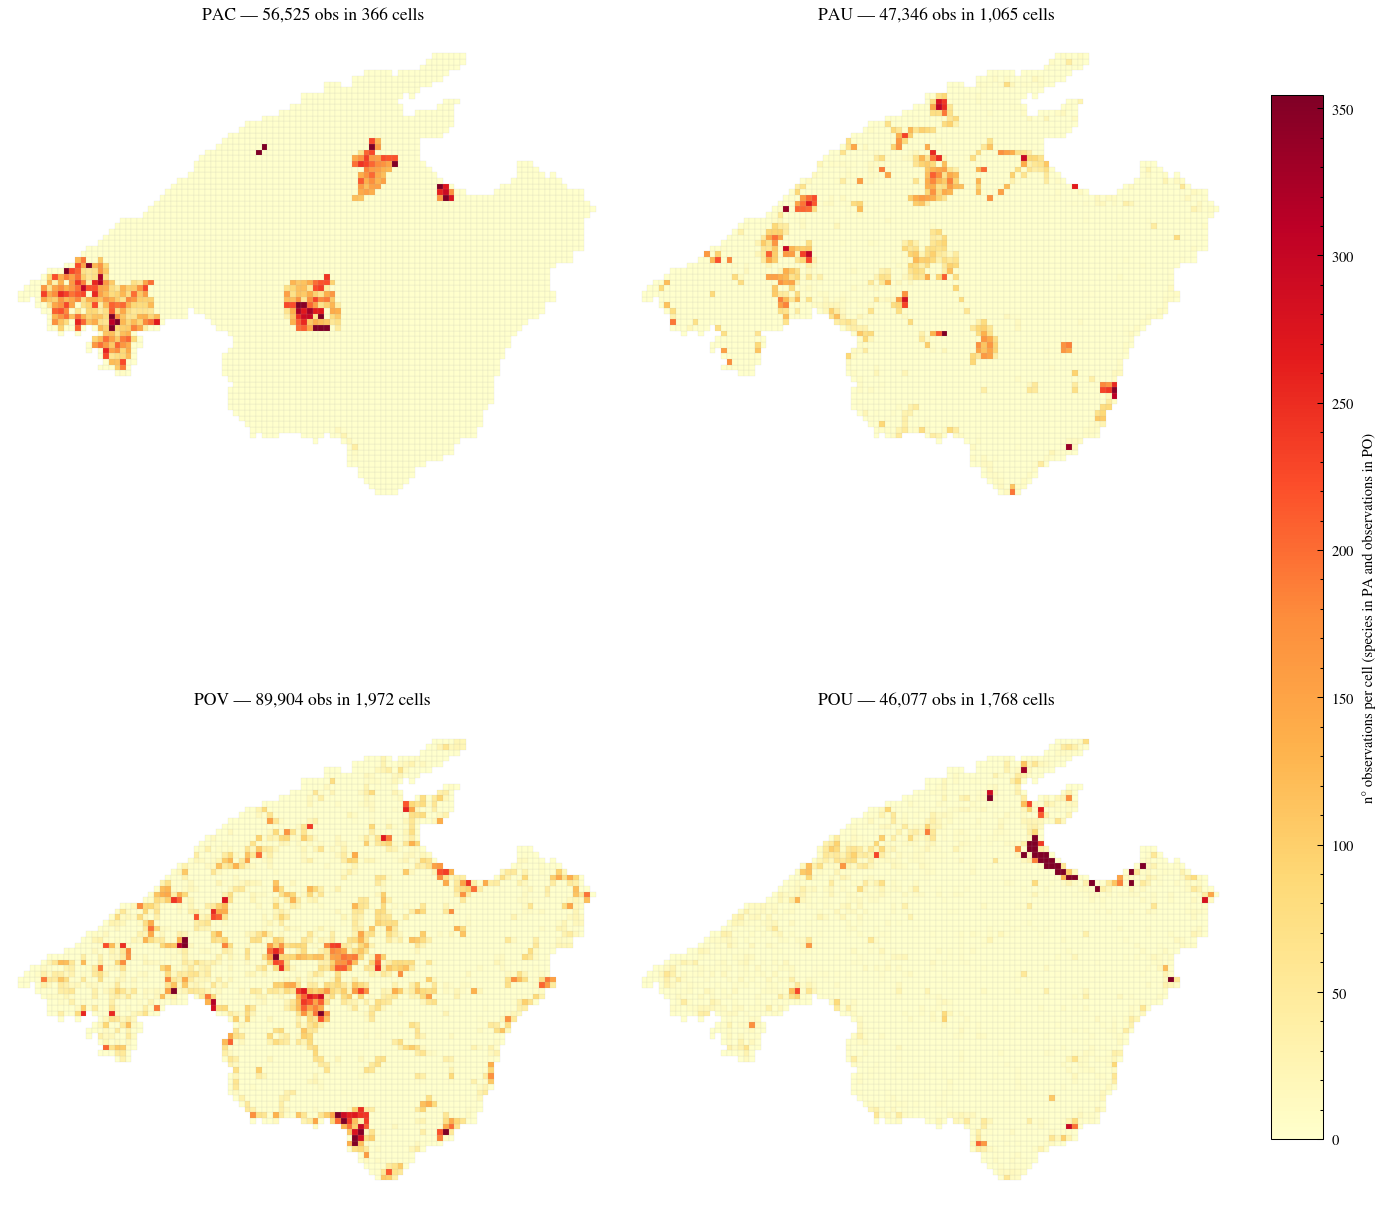
\includegraphics[width=1\linewidth]{figures/grid_density_by_source.png}
    \caption{Map representing species density in PA and observations density in PO in a a grid of 1x1km. }
    \label{fig:Figure1Map}
\end{figure}

\begin{figure}
    \centering
    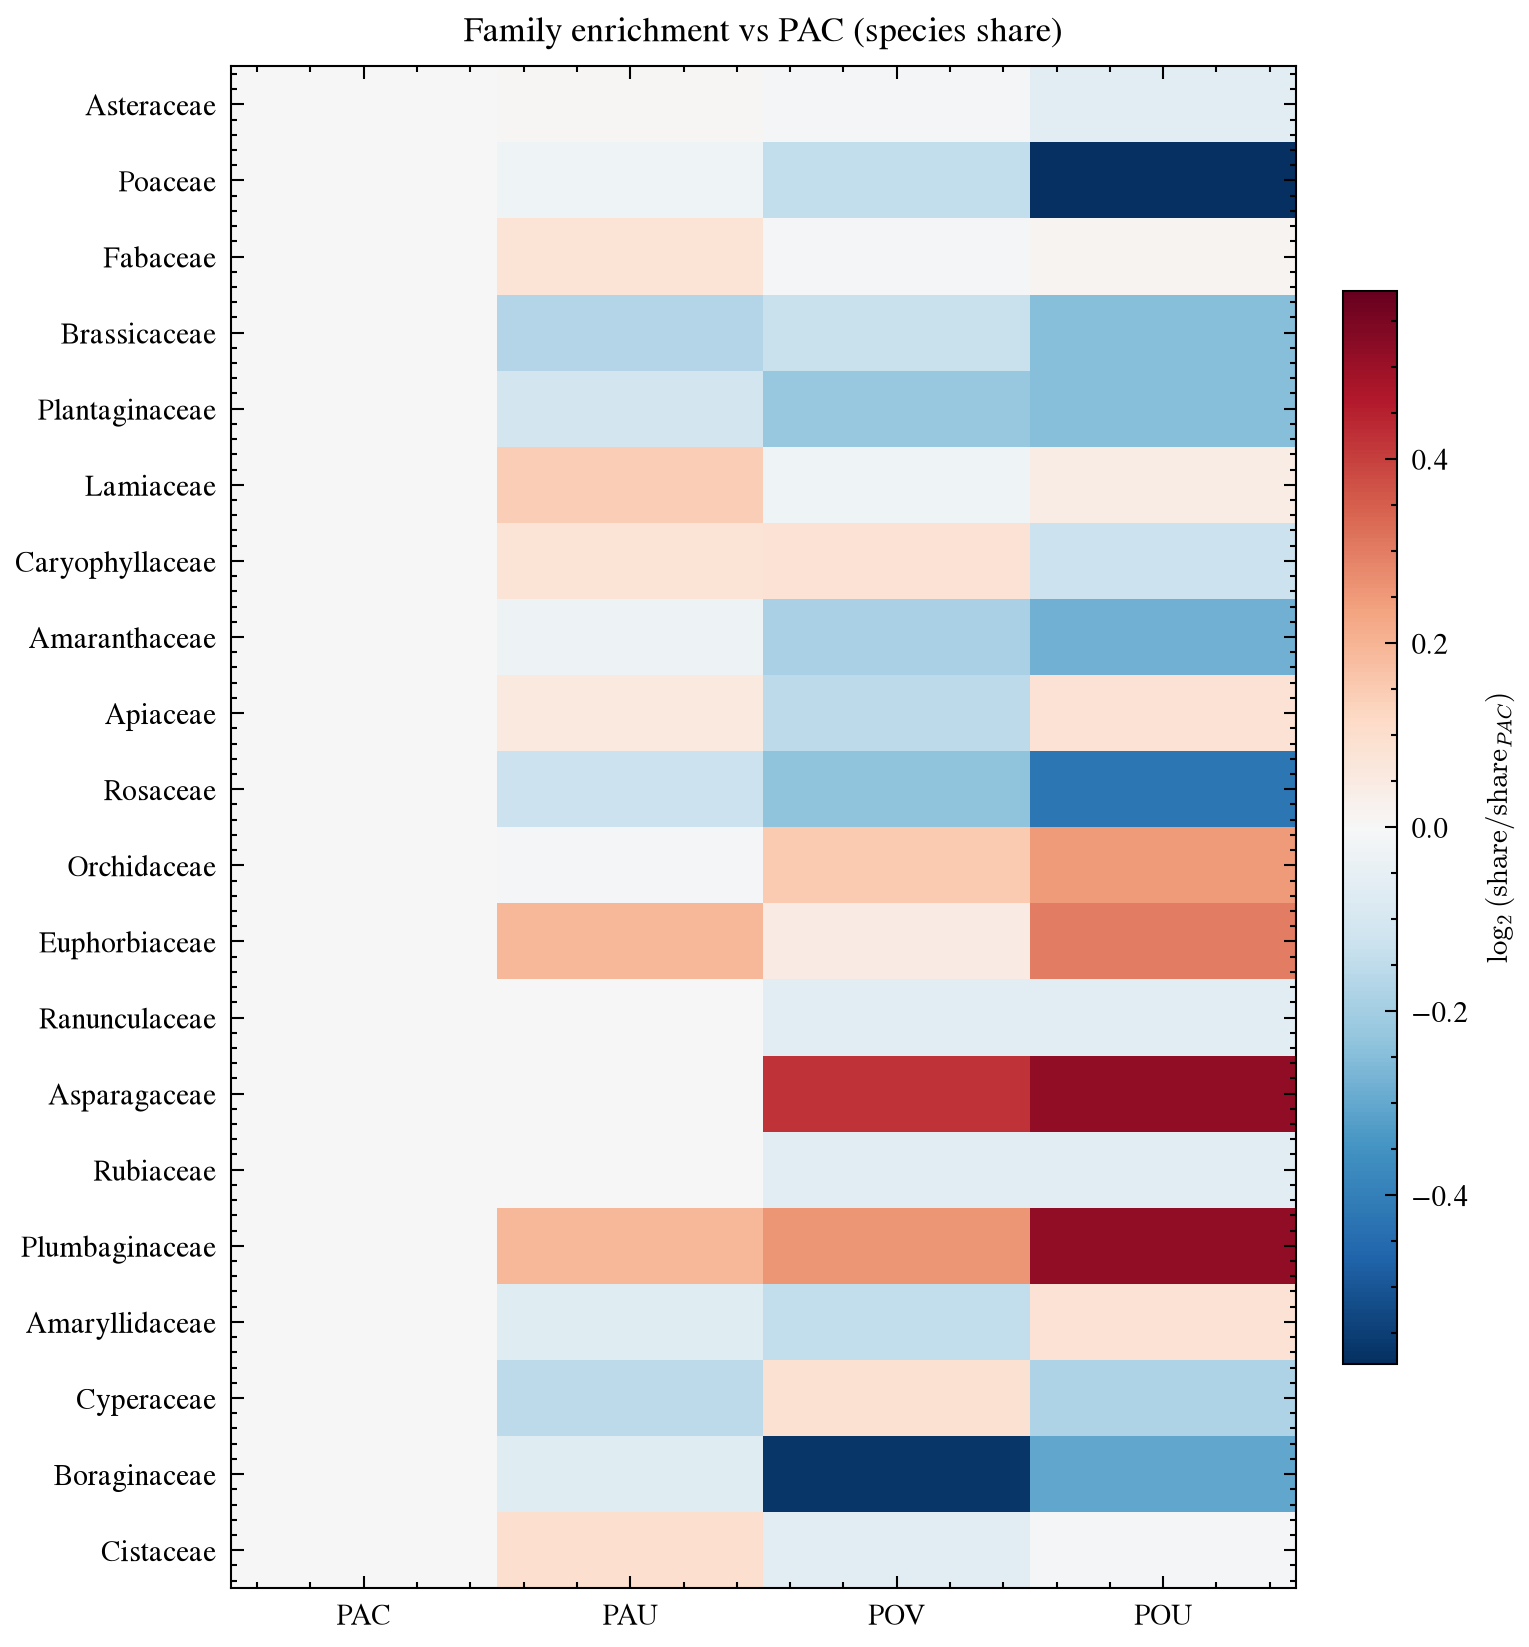
\includegraphics[width=0.92\linewidth]{figures/taxonomy_by_source_family.png}
    \caption{Species-share enrichment by family relative to PAC ($\log_2(\mathrm{share}/\mathrm{share}_{\mathrm{PAC}})$) for the 20 families with most species in PAC. PAU closely matches PAC; POV/POU show clearer taxonomic skew (e.g.\ Poaceae under-represented in POU).}
    \label{fig:taxonomy_family}
\end{figure}




\begin{figure}
    \centering
    \includegraphics[width=1\linewidth]{../../output/curated/rarity_by_source.png}
    \caption{Q1: share of species by PAC prevalence bin (rare $<$5\%, medium 5--30\%, common $>$30\%) across observation levels (curated taxon set).}
    \label{fig:rarity_by_source}
\end{figure}

\begin{figure}
    \centering
    \includegraphics[width=1\linewidth]{../../output/curated/common_pac_in_po_rarification.png}
    \caption{Q1b: among PAC-common species, ratio of PAC cell prevalence to source cell prevalence (values $>$1 = species looks rarer in that source). Cell-grain comparison.}
    \label{fig:rarification}
\end{figure}

\begin{figure}
    \centering
    \includegraphics[width=1\linewidth]{../../output/curated/species_accumulation_mix.png}
    \caption{Q3 inventory: unique species and PAC-rare recovery under factorial 0/50/100\% mixes of PAU/POV/POU cells.}
    \label{fig:inventory_mix}
\end{figure}

\begin{figure}
    \centering
    \includegraphics[width=1\linewidth]{../../output/curated/sampling_effort_auc_by_prevalence.png}
    \caption{Q1/Q2 SDM: learning curves (mean PAC AUC) by train source and PAC prevalence bin; point vs grouped (curated). Paths under \texttt{output/curated/}.}
    \label{fig:sampling_effort_curated}
\end{figure}

\begin{figure}
    \centering
    \includegraphics[width=1\linewidth]{../../output/curated/optimal_model_auc_grouped.png}
    \caption{Q2/Q3 SDM: factorial mixes of PAU/POV/POU at cell grain (grouped), mean per-species AUC on PAC (curated).}
    \label{fig:optimal_mix_curated}
\end{figure}


\subsection{Effectiveness }

\section{Discussion}


Previous studies have shown increased accuracy using Data Fusion techniques, although they also suggest avoiding simple pooling \cite{fletcher2019practical}

Weighting joint likelihood functions is a practical way to place greater emphasis on one data source \cite{fletcher2019practical}.

\subsection{Implications for rare species}

SDMs face challenges when assessing the distribution of rare species because they are hardly captured by most survey systems, suggesting the potential benefitial use of hierarchical SDMs \cite{https://doi.org/10.1111/gcb.16114}

Previous wroks observed that GBIF data systematically failed to consistently improve predictive performance due to limited observations and spatial biases \cite{Datafusion2025}, while others observed increased accuracies when including similar data sources  and interestingly observing null increases in accruacy for common species \cite{atsumi2024boosting}

For rare species, predictive performance was improved by multi-species modeling, with shared ecological and spatial structures being captured more effectively \cite{Datafusion2025}

Information of public repositories, including GBIF, is using for threatened species assesment, while previous works proved that expert curation of this data lead to differential threatening categories for evaluated species (\cite{panter2020clean})

\subsection{Limitations}

Data curation has been proposed to be more efficient than fieldwork ()
Data imbalance between PA and PO is a known challenge of SDMs \cite{Grattarola2023}

We must consider the differential effort/quality and expertise necessary to produce one observation of PA, POV and POU. PAC requires extensively visitng the study area by an experimented researcher, while POV requires generating point data at lower frequancy visits by expertos or validating POU by experts. 

\section{Conclusions}

\section{References}



\section{Notes}

\begin{itemize}
    \item Should weights of PAU take into account the number of species in that point? PAU with 2 species is not as good in terms of quality as PAU with 200 species (although in some cases structural constraints such as a lot of sea area can lead to real low diversity values)
    \item In GBIF, there are values with enormous coordinateUncertainty. Currently, all values with uncertainties higher than 1000m have been omitted, but it can also be considered as low quality values and be maintained if properly handled
    \item There is a 5th type of data, inventories at high-resolution, which could be used to estimate species diversity based on other species diversity. The volume of that type of data in Mallorca is very limited. 

Frases cvlave para discutir

\textbf{1. El valor de la Fusión de Datos (Integrated Species Distribution Models - IDMs)}

\begin{itemize}
        \item \textbf{Frase clave:} "Our results demonstrate that Integrated Species Distribution Models (IDMs) effectively capitalize on the broad spatial coverage of opportunistic GBIF records while maintaining the statistical rigor provided by true absences from exhaustive floristic inventories."
        \item \textit{Por qué funciona:} Esta frase establece inmediatamente el éxito de tu metodología híbrida, destacando que has logrado unir el volumen masivo de datos globales con la calidad estructurada de los catálogos regionales.
\end{itemize}
\textbf{2. Mitigación de Sesgos Espaciales y Taxonómicos}

\begin{itemize}
        \item \textbf{Frase clave:} "By incorporating validated citizen science data and structured plots, our data fusion approach successfully mitigates the spatial and taxonomic biases—such as the overrepresentation of conspicuous species near accessible infrastructures—inherent to unstructured presence-only datasets."
        \item \textit{Por qué funciona:} Aborda directamente el problema histórico de usar solo datos crudos de GBIF (el sesgo humano de muestreo cerca de carreteras o centros de investigación) y justifica cómo tu modelo corrige estas distorsiones.
\end{itemize}
\textbf{3. Superioridad de las Ausencias Reales sobre las Pseudoausencias}

\begin{itemize}
        \item \textbf{Frase clave:} "Unlike traditional presence-only models that rely heavily on analytically generated pseudo-absences, the integration of structured presence-absence data from regional floras provides a cleaner ecological signal, significantly reducing model uncertainty and preventing the overestimation of the species' bioclimatic niche."
        \item \textit{Por qué funciona:} Destaca la importancia metodológica de tu enfoque. Las pseudoausencias aleatorias pueden generar falsos negativos o distorsionar los límites del hábitat, mientras que tus datos exhaustivos anclan el modelo a una realidad ecológica comprobable.
\end{itemize}
\textbf{4. El rol complementario de la Ciencia Ciudadana Validada}

\begin{itemize}
        \item \textbf{Frase clave:} "Citizen science platforms, when subjected to rigorous taxonomic validation, act as a crucial complementary source, filling critical geographical gaps in undersampled regions and expanding the environmental gradients captured by formal academic inventories."
        \item \textit{Por qué funciona:} Legitima el uso de la ciencia ciudadana en la academia. Demuestra que, tras un filtrado de calidad, estas plataformas aportan presencias únicas que superan las barreras de tiempo y financiamiento de los muestreos tradicionales.
\end{itemize}
\textbf{5. Implicaciones aplicadas para la Macroecología y Conservación}

\begin{itemize}
        \item \textbf{Frase clave:} "Ultimately, bridging the dichotomy between massive unstructured observations and localized exhaustive surveys provides a more robust, ecologically coherent, and transferable framework for plant biodiversity monitoring and conservation planning under data-deficient scenarios."
        \item \textit{Por qué funciona:} Cierra la discusión proyectando la utilidad práctica de tu estudio, sugiriendo que esta metodología híbrida debería ser el nuevo estándar para evaluar el riesgo de extinción y planificar estrategias de conservación fiables.
\end{itemize}

    \
\end{itemize}

\end{document}

